\chapter{Metodologia}
\label{CHP:MET}

Neste cap�tulo s�o descritos os ambientes utilizados no desenvolvimento, avalia��o e teste da ferramenta proposta, chamada de MDiag. Algumas caracter�sticas importantes da implementa��o, que garantem a efic�cia do diagn�stico, s�o apresentadas na Se��o \ref{SEC:DES}. Um sistema autom�tico de inser��o de falhas desenvolvido para valida��o do MDiag atrav�s de simula��o, � detalhado na Se��o \ref{SEC:SIM}. Por fim, � descrito o procedimento de testes em ambientes reais.

    %%% Se��o 3.1:
    \section{Ambiente de Desenvolvimento e Teste}

Para o desenvolvimento deste trabalho, foram utilizados diversos tipos de computadores a fim de garantir compatibilidade com a maior variedade poss�vel de plataformas. Sistemas variando desde kit de desenvolvimento de sistema embarcado at� servidores de grande porte com distribui��es Linux variadas. Todas as m�quinas utilizadas, com exce��o de um computador pessoal do autor, fazem parte do acervo do \ac{LESC} da \ac{UFC}.

Nenhum tipo de bibliotecas, al�m das padr�es do Linux, foram necess�rias durante o desenvolvimento, pois, para favorecer a portabilidade, a ferramenta utiliza apenas funcionalidades presentes no pr�prio \emph{kernel} do Linux, a partir da vers�o 2.6.9.

Para simular as falhas em mem�ria, foi utilizada uma abordagem baseada em \cite{PETRU:2002} (descrita com detalhes na se��o \ref{SEC:SIM}). Um \emph{software} de \emph{debug} com capacidade de estabelecer \emph{breakpoints} em n�vel de \emph{hardware} foi utilizado para interromper a execu��o do teste no momento desejado e escrever um valor de erro na mem�ria, simulando qualquer tipo de falha. O \emph{software} utilizado foi o \ac{GDB}, uma das mais consagradas ferramentas de \emph{debug} para Linux.

Foram realizados testes com mem�rias defeituosas reais e os resultados foram comparados aqueles obtidos por outras ferramentas de diagn�stico do mercado. Os componentes e o procedimento desta avalia��o s�o detalhados na Se��o \ref{SEC:REAL} 
    %%% Se��o 3.2:
    \section{Implementa��o do MDiag}
\label{SEC:DES}

Para o desenvolvimento de um diagn�stico que atua sobre um sistema operacional, alguns cuidados precisam ser tomados para garantir a efic�cia dos testes. Como visto na Se��o \ref{SEC:LINUXMM}, cada acesso � mem�ria passa por uma s�rie de abstra��es at� chegar ao \emph{hardware}. Isto pode acarretar falsos resultados ou inefici�ncias no diagn�stico.

Por exemplo, durante o teste o \emph{kernel} pode guardar parte da mem�ria alocada no \emph{swap}, enquanto o restante � testado. Depois, essas p�ginas podem ser recuperadas e a parte testada pode ser armazenada. A por��o resgatada pode estar em qualquer lugar do espa�o f�sico destinado ao processo, at� mesmo no lugar da por��o que j� foi testada, causando uma dupla checagem nestas c�lulas e deixando de testar outras.

Por isso o MDiag executa uma s�rie de procedimentos, mostrados na Figura \ref{FIG:FLUXO}, antes de executar os algoritmos de teste. O conjunto de opera��es desde a limpeza do \emph{cache} at� a aloca��o, de fato, da mem�ria � um mecanismo projetado neste trabalho chamado de pol�tica de aloca��o de mem�ria do MDiag, que visa maximizar quantidade de mem�ria coberta pelo diagn�stico sem comprometer estabilidade do sistema.

\begin{figure}[!ht]
\centering
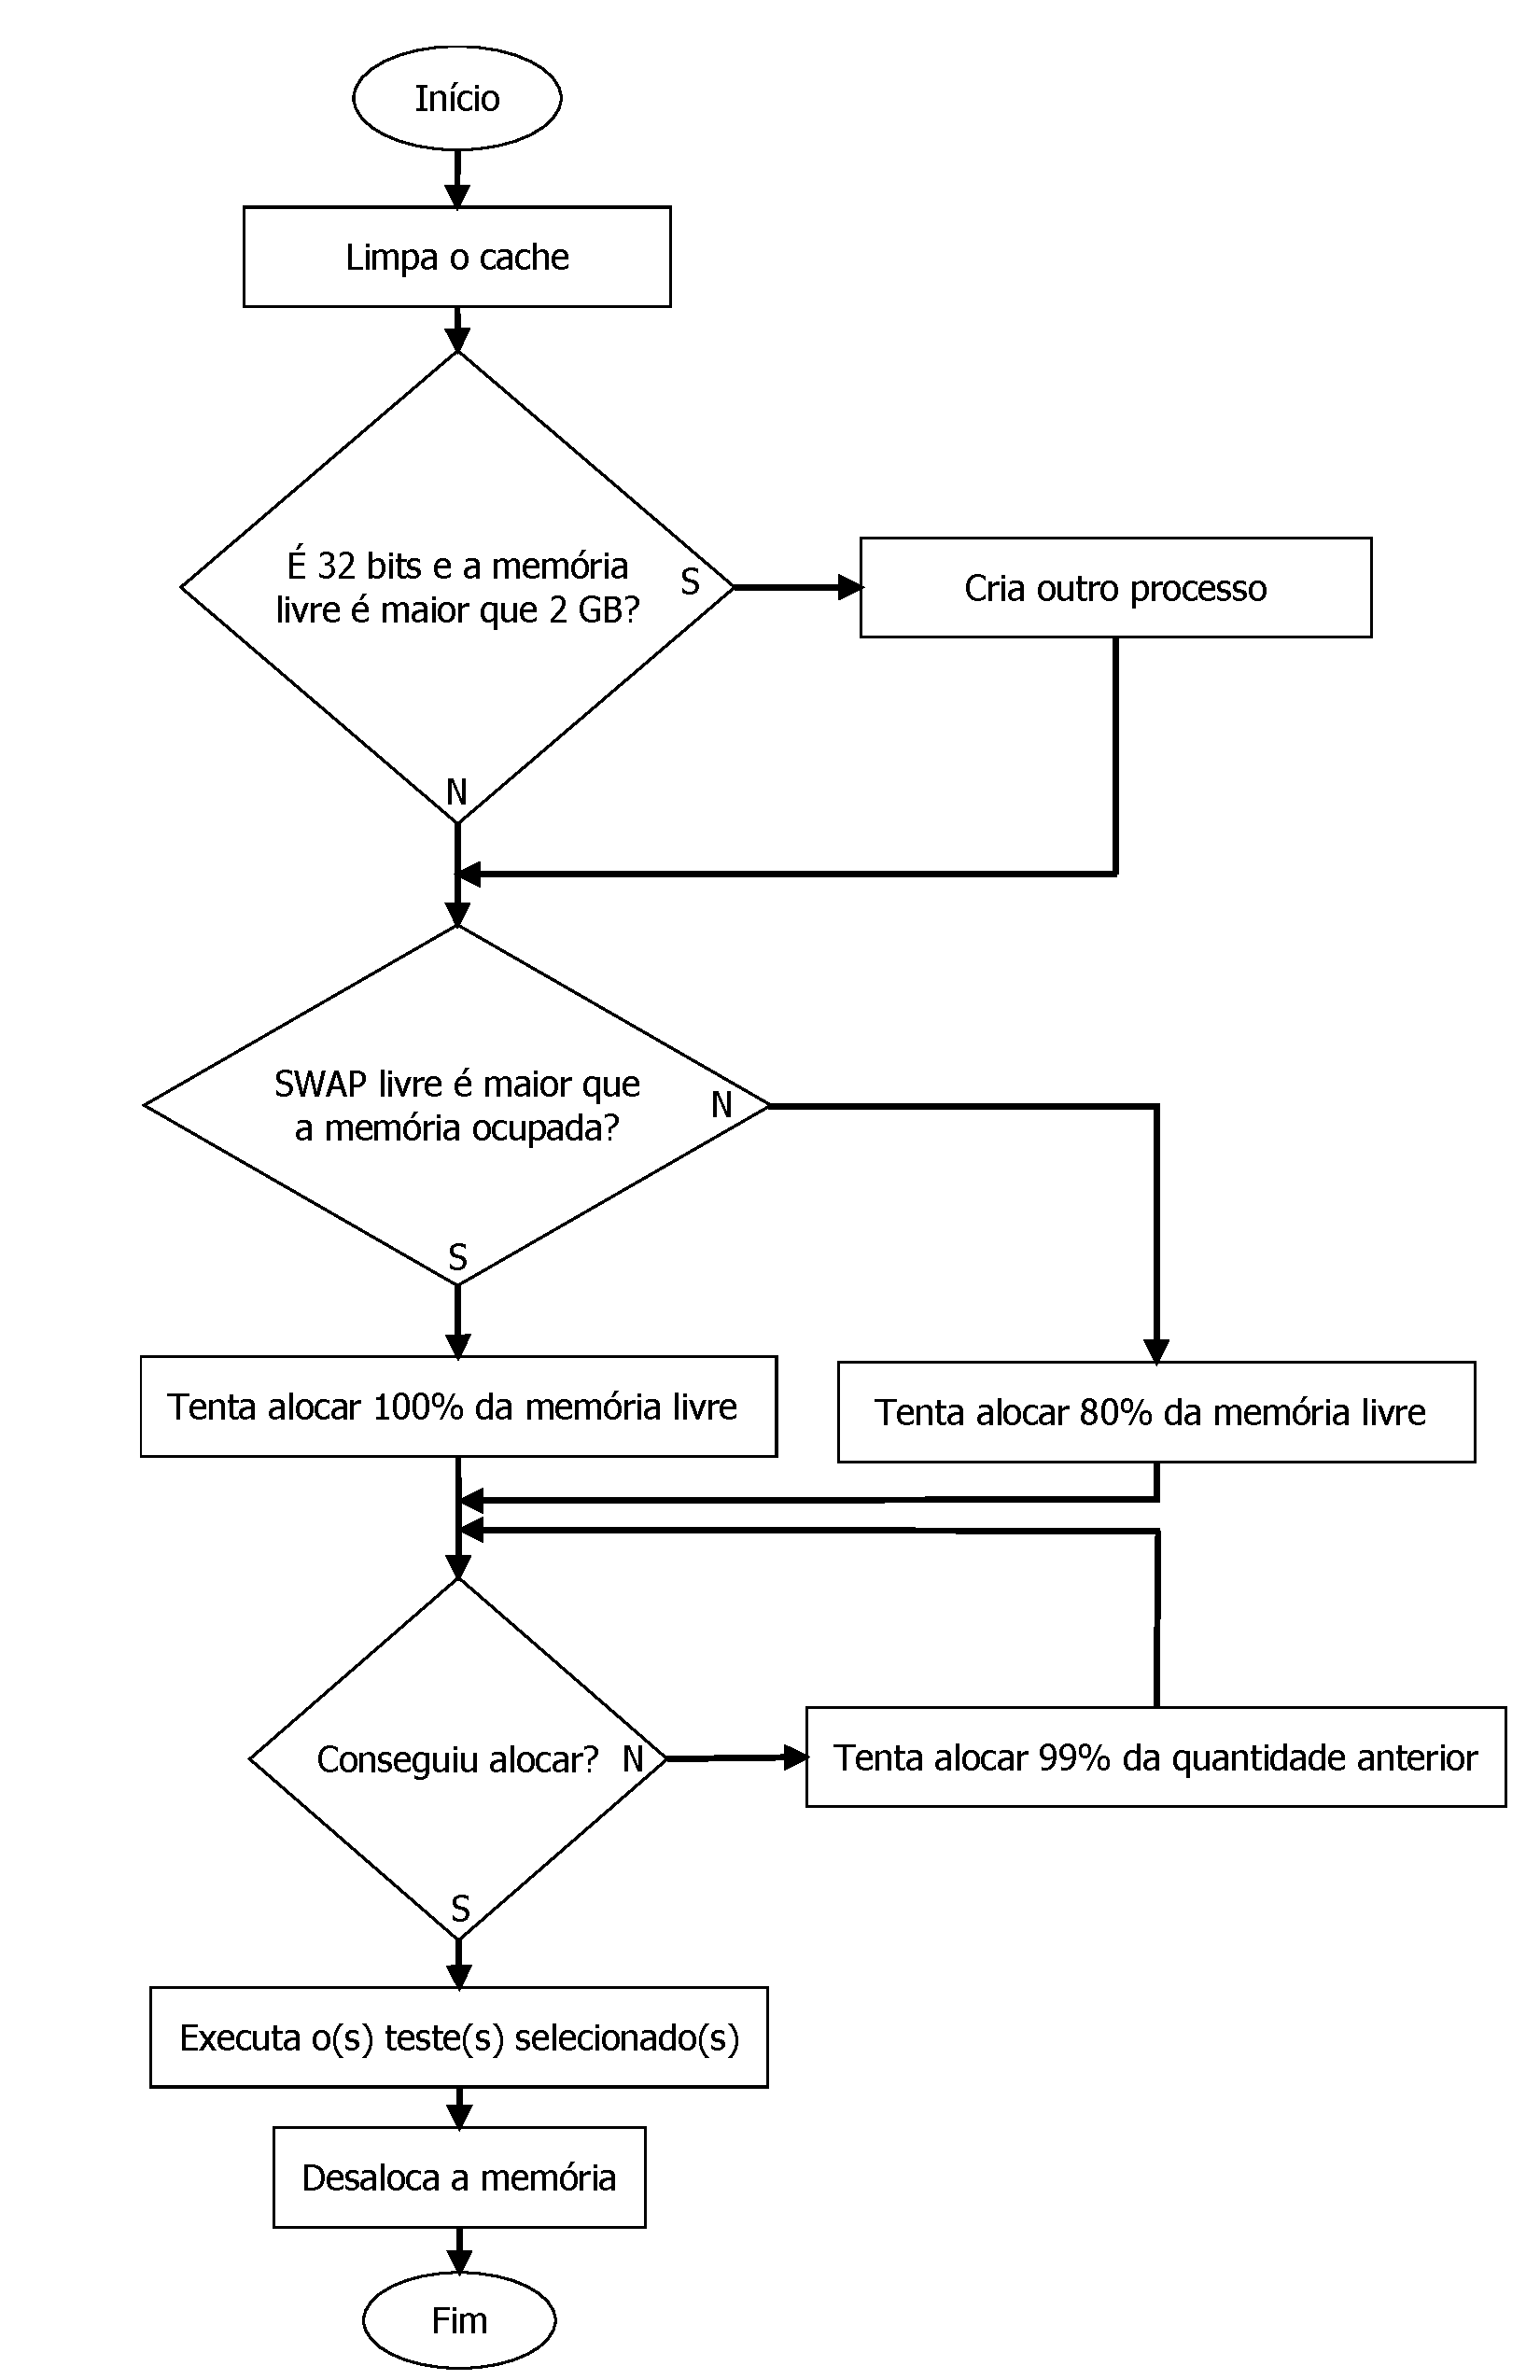
\includegraphics[width = 0.9 \linewidth]{figs/fluxo.pdf}
\caption[Fluxo de execu��o do MDiag]{Fluxo de execu��o do MDiag.} \label{FIG:FLUXO}
\end{figure}

\subsection{Pol�tica de aloca��o de mem�ria}

� imposs�vel que um diagn�stico implementado como um aplicativo, que executa sobre um Linux sem altera��es nos mecanismos de prote��o do \emph{kernel}, possa testar toda a mem�ria instalada, isto porque certa quantidade de mem�ria, chamada de �rea do sistema, � reservada para o pr�prio \ac{SO} guardar suas estruturas de dados, executar e gerenciar as aplica��es. Muitas outras aplica��es executando em paralelo consomem outras por��es da �rea restante. No entanto, quanto mais mem�ria for testada, mais efetivo o diagn�stico ser�, possibilitando detectar mais falhas. Por isso a pol�tica de aloca��o foi tratada com bastante crit�rio durante este projeto.

O Linux possui, simplificadamente, tr�s estados de mem�ria: alocada, em \emph{cache} e livre. O mecanismo de \emph{cache} foi explicado na Se��o \ref{SEC:LINUXMM}. Como foi dito, ap�s algum tempo em opera��o a tend�ncia � que apenas uma pequena parte da mem�ria permane�a realmente livre, a maior parte estar� sendo utilizada como \emph{cache} ou alocada para algum processo. O MDiag aloca apenas a por��o livre da mem�ria, para evitar que o sistema sofra de \ac{OOM}. Por isso o primeiro passo � a limpeza do \emph{cache}, liberando qualquer parte dispens�vel da mem�ria e, consequentemente, aumentando a �rea testada.

Em seguida h� o tratamento de uma limita��o de sistemas 32 bits. Nestes sistemas o endere�amento m�ximo acess�vel por um processo � de 4 GB. O Linux possui um mecanismo chamado \emph{HighMemory} que permite que um \emph{kernel} 32 bits acesse mais de 4 GB de mem�ria f�sica em um \emph{hardware} 64 bits. No entanto, isto permite apenas que mais processos sejam alocados por vez, mas cada um deles ainda ter� acesso a, no m�ximo, 4 GB de mem�ria. Al�m disto, dentro deste espa�o h� uma �rea reservada para que o \emph{kernel} controle aquele processo, al�m de �reas utilizadas como mem�ria de c�digo e pilha. Assim, o m�ximo que uma aplica��o consegue alocar para uso pr�prio varia tipicamente em torno de 3 GB.

Para contornar esta limita��o, o MDiag verifica se o sistema � 32 bits e se a mem�ria livre � maior que 2 GB. Neste caso, o programa se duplica em dois processos id�nticos, mas totalmente independentes (\emph{fork}). Isto faz com que dois testes com os mesmos par�metros sejam executados simultaneamente, cada um fazendo sua pr�pria tentativa de aloca��o e ampliando a mem�ria total testada. � claro que ainda assim pode acontecer de nem toda a mem�ria livre ser alocada, mas o limite � dobrado para aproximadamente $6 GB$.

A aloca��o de mem�ria no MDiag � um processo de duas etapas. Primeiramente h� a aloca��o em si (\emph{malloc}), isto �, solicitar ao \emph{kernel} uma por��o de mem�ria de tamanho fixo para ser utilizada pela aplica��o. Uma vez concedida, esta regi�o deve ser travada (\emph{mlock}). Isto significa que o processo indica ao \emph{kernel} que aquela regi�o de mem�ria n�o pode ser armazenada em \emph{swap}, garantindo que tudo o que foi alocado esteja realmente na mem�ria f�sica da m�quina. Se uma das etapas receber resposta negativa do \emph{kernel}, o processo de aloca��o falhou. Neste caso, � feita uma nova tentativa de aloca��o   com 99\% da quantidade pretendida anteriormente. Este processo se repete at� que se obtenha sucesso ou at� que a quantidade pretendida se torne abaixo de 10 MB.

Outra medida tomada, na pol�tica de aloca��o, para evitar \ac{OOM} � de n�o alocar toda a mem�ria virtual do sistema. Isto � feito assegurando-se de que h� espa�o suficiente no \emph{swap} para armazenar toda a mem�ria atualmente em uso, se necess�rio. Caso contr�rio, apenas 80\% da mem�ria livre � alocada. Este n�mero foi alcan�ado de forma emp�rica com testes em diversas m�quinas reais com diferentes distribui��es Linux, diferentes tamanhos de mem�ria e diferentes perfis de uso (muitos processos ou poucos processos). � o maior percentual em que se notou um baix�ssimo risco de \ac{OOM}.

Ap�s passar por toda a pol�tica de aloca��o, finalmente os testes podem ser aplicados sequencialmente � regi�o de mem�ria alocada.

\subsection{Algor�tmos Implementados}

Neste trabalho foram utilizados seis algoritmos, permitindo realizar testes mais r�pidos ou testes com maior cobertura de falhas. Foram escolhidos os algoritmos de maior reconhecimento na literatura, citados em praticamente todos os artigos e livros da �rea, com uso consagrado na ind�stria e com resultados comprovados em an�lises comparativas de testes de mem�ria \cite{RIEDEL:1995,RAGHURAMAN:2005}.

\subsubsection{March C-}

O March C- � um teste ainda muito utilizado por possuir duas caracter�sticas bastante fortes: entre os testes do tipo marchante, � um dos que possui maior cobertura de falhas; � um teste r�pido, com complexidade de apenas $10 N$ opera��es.

No MDiag foi implementada tamb�m a varia��o proposta por \cite{ADAMS:2003}, chamada de Enhanced March C- e descrita na tabela \ref{TAB:EMARCHC-}. Esta forma melhorada do March C- � mais lenta, com $8N$ opera��es a mais, mas possui uma cobertura de falhas um pouco maior.

As descri��es destes testes j� foram apresentadas na se��o \ref{SEC:TESTES}, especialmente nas Tabelas \ref{TAB:MARCHC-} e \ref{TAB:EMARCHC-}.

\subsubsection{March G}

Da s�rie de testes March, o que obteve melhores resultados at� hoje foi proposto por \cite{VANDEGOOR:1998}. O March G (tabela \ref{TAB:MARCHG}) introduz um novo tipo de elemento al�m das escritas e leitura convencionais. � uma pausa entre as sequ�ncias, que possibilita a detec��o de falha de reten��o (\emph{data retention fault}).

\begin{table}[!ht]
\caption{\emph{March G pattern.}}
\centering
\label{TAB:MARCHG}
\begin{tabular}{| c | l r |}
\hline
1 & W0 & $\Updownarrow$ \\
2 & R0, W1, R1, W0, R0, W1 & $\Uparrow$ \\
3 & R1, W0, W1 & $\Uparrow$ \\
4 & R1, W0, W1, W0 & $\Downarrow$ \\
5 & R0, W1, W0 & $\Downarrow$ \\
6 & pausa & \\
7 & R0, W1, R1 & $\Updownarrow$ \\
8 & pausa & \\
9 & R1, W0, R0 & $\Updownarrow$ \\
\hline
\end{tabular}
\end{table}

\subsubsection{Papachristou}

Para um teste mais completo, o algoritmo adotado foi o proposto por \cite{PAPACHRISTOU:1985}. � um teste longo, que demanda $38N+24N\log_2(N)$ opera��es, o equivalente a $16,9$ minutos para testar 1 GB ou mais de uma hora para testar 4 GB de mem�ria nas condi��es da tabela \ref{TAB:TEMPOS}. Apesar de ser um padr�o antigo, sua abrang�ncia na detec��o de falhas vem sendo confirmada por trabalhos mais recentes \cite{RIEDEL:1995} \cite{PETRU:2002}.

No MDiag, foram implementados os algoritmos parcial e completo de Papachristou. Ambas as varia��es foram apresentados na Se��o \ref{SEC:TESTES}.

Todos os algoritmos at� aqui foram implementados tomando como c�lulas os bytes da mem�ria, portanto cada c�lula possui 8 bits de tamanho. Os estados 0 e 1 em que a c�lula pode estar representam um padr�o qualquer de $00_h$ a $FF_h$ e seu inverso (complemento bit-a-bit), permitindo que os testes detectem erros mais variados. Por exemplo, o March C- � capaz de detectar \emph{idempotent} \ac{CF} se utilizado o estado 0 como o valor $00_h$ e, por consequ�ncia, estado 1 como o valor $FF_h $, mas n�o � capaz de detectar \emph{inversion} \ac{CF}. J� com a utiliza��o do padr�o $55_h$ como o estado 0 e seu inverso $AA_h$ como estado 1, ocorre exatamente o oposto.

\subsubsection{MT}

O mais recente dentre os algoritmos implementados � o MT (Tabela \ref{TAB:MT}). � um teste que possui uma cobertura t�o boa quanto Papachristou, mas de complexidade $O(N)$.

Como visto em sua descri��o na Se��o \ref{SEC:TESTES}, este teste trabalha com base na disposi��o matricial das c�lulas da mem�ria. Desta forma, sua implementa��o foi um pouco diferente dos demais. Primeiramente, para manter a estrutura matricial pressuposta pelo algoritmo, as c�lulas foram tomadas como sendo os \emph{bits} e n�o mais o \emph{bytes} da mem�ria. Assim, tem-se uma matriz $8 \times N$ de c�lulas, podendo-se aplicar os padr�es de fundo da tabela $I_1$ a $I_6$ da \ref{TAB:MTBACKGROUNDS}. Da mesma forma, devido a utiliza��o de padr�es j� bem definidos no algoritmo, este teste n�o permite escolher o que os estados 0 e 1 significam, mesmo porque as c�lulas agora s�o apenas bits, que s� assumem os valores 0 e 1.

\subsection{Desaloca��o da Mem�ria}

O pr�ximo passo, consiste na desaloca��o de toda a mem�ria. Da mesma forma que a aloca��o, este tamb�m � um processo de duas etapas. Primeiro a mem�ria � destravada, para ent�o ser desassociada do processo.

� importante garantir que a mem�ria seja devidamente desalocada, mesmo no caso do programa ter sua execu��o interrompida, seja pelo usu�rio ou pelo \emph{kernel}. Isto porque a quantidade de mem�ria reservada para o diagn�stico representa uma por��o significativa do total dispon�vel, al�m da regi�o estar travada, n�o podendo nem mesmo ser despejada para \emph{swap}.

O MDiag utiliza um manipulador de sinal (\emph{signal handler}) que nada mais � que uma fun��o a ser executada sempre que o \emph{kernel} enviar certo sinal. Este manipulador monitora um sinal do \emph{kernel} que � disparado sempre que h� uma tentativa de interrup��o ao processo. O manipulador deve ser r�pido, pois o \emph{kernel} envia este sinal como aviso de que o programa ser� fechado, e caso o processamento n�o cesse, o \emph{kernel} poder� matar o processo abruptamente. 
    %%% Se��o 3.3:
    \section{Inser��o de Falhas}
\label{SEC:SIM}

A fim de comprovar a efic�cia dos testes, foi desenvolvido um ambiente de valida��o autom�tico com inser��o de falhas via \emph{debugging}.

O m�todo utiliza elementos de \emph{debugging} presente na maioria dos processadores atuais. O \ac{GDB} foi usado como interface de \emph{software} para explorar esses recursos do \emph{hardware}. Foram utilizadas principalmente duas estruturas: \emph{breakpoint} e \emph{watchpoint}. O primeiro � apenas um ponto de parada na execu��o do programa, congelando-o at� que seja dado o comando para continuar. O segundo � similar ao primeiro, mas o crit�rio de parada n�o est� associado a um ponto espec�fico do c�digo, mas a uma vari�vel, fun��o ou posi��o da mem�ria. A execu��o � interrompida cada vez que houver uma tentativa de leitura ou escrita no endere�o monitorado.

\subsection{Falhas simuladas}

As falhas inseridas foram limitadas aos erros mais desafiadores para os algoritmos de teste de mem�ria, eliminando redund�ncias no sistema e otimizando o tempo de valida��o. Os modelos mais simples, como \ac{SAF} e \ac{TF}, n�o foram levados em considera��o, pois todos os algoritmos apresentados possuem cobertura de 100\% na sua detec��o \cite{RIEDEL:1995} \cite{PETRU:2002} \cite{RAGHURAMAN:2005}. Foram escolhidas apenas falhas representativas, em que � esperado que os testes n�o possam detectar todas as varia��es poss�veis.

Os modelos de falha que apresentam maior dificuldade na detec��o s�o os de acoplamento. Tanto os \ac{CF} simples, como \ac{NPSF} ou, de forma mais geral, falhas de \emph{k-coupling}. Para a valida��o foram inseridas falhas do tipo \emph{idempotent} \ac{CF}, \emph{inversion} \ac{CF} e \emph{3-coupling fault}. Estas foram aplicadas apenas entre c�lulas vizinhas, pois, al�m de ser a situa��o mais comum encontrada em mem�rias reais \cite{PETRU:2002}, cobre as tr�s ordena��es poss�veis de acoplamento: a v�tima (c�lula que sofre transi��o err�nea) acima da agressora (c�lula que dita o estado da v�tima), a v�tima abaixo da agressora e a v�tima e a agressora no mesmo byte.

Da mesma forma, para eliminar redund�ncia no sistema e otimizar o tempo de valida��o, os \emph{bits} utilizados foram limitados aos mais representativos. As falhas se combinam apenas entre os bits 0, 1, 6 e 7 de cada \emph{byte}. Assim os casos cobertos s�o: \emph{bits} nas bordas da c�lula, \emph{bits} fora das bordas, \emph{bits} vizinhos, \emph{bits} distantes, v�tima a direita da agressora e v�tima a esquerda da agressora.

De forma mais simples, cada falha foi inserida com todas as combina��es entre acoplado e acoplador nos bits destacados na figura \ref{FIG:CELULAS_FALHAS}.

\begin{figure}[!ht]
\centering
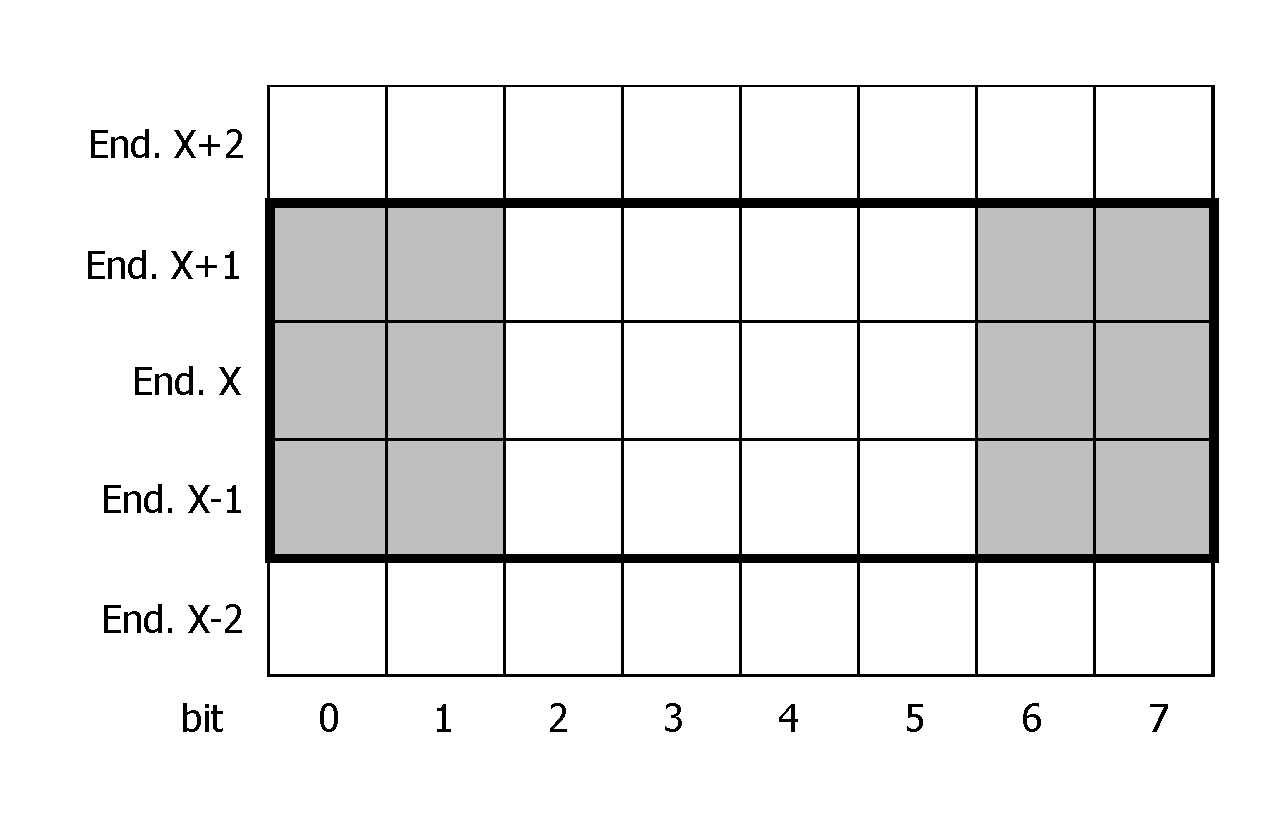
\includegraphics[width = 0.7 \linewidth]{figs/celulas_falhas.pdf}
\caption[Bits atingidos pela inser��o de falhas]{Bits atingidos pela inser��o de falhas.} \label{FIG:CELULAS_FALHAS}
\end{figure}

Para cada modelo simulado, as combina��es poss�veis s�o dadas por: $(b \cdot 3 - 1) \cdot b$ para acoplamento entre duas c�lulas e $(b \cdot 3 - 2) \cdot (b \cdot 3 - 1) \cdot b$ para tr�s, com $b$ sendo a quantidade de \emph{bits} em que as falhas podem ocorrer em  cada \emph{byte}. Para a falha \emph{3-coupling fault} h� duas possibilidades: que a c�lula v�tima sofra transi��o quando uma das outras for escrita e a terceira esteja no estado 0 ou quando esta esteja no estado 1.

Portanto, o total de combina��es de falhas geradas para b = 4 �:

$2 \cdot (4 \cdot 3 - 1) \cdot 4 = 88$

$+$

$2 \cdot (4 \cdot 3 - 2) \cdot (4 \cdot 3 - 1) \cdot 4 = 880$

$= 968$ falhas.

\subsection{Sistema de inser��o de falhas}

A Figura \ref{FIG:FLUXO_SIM} mostra os passos do sistema de inser��o de falhas elaborado para validar o MDiag.

\begin{figure}[!ht]
\centering
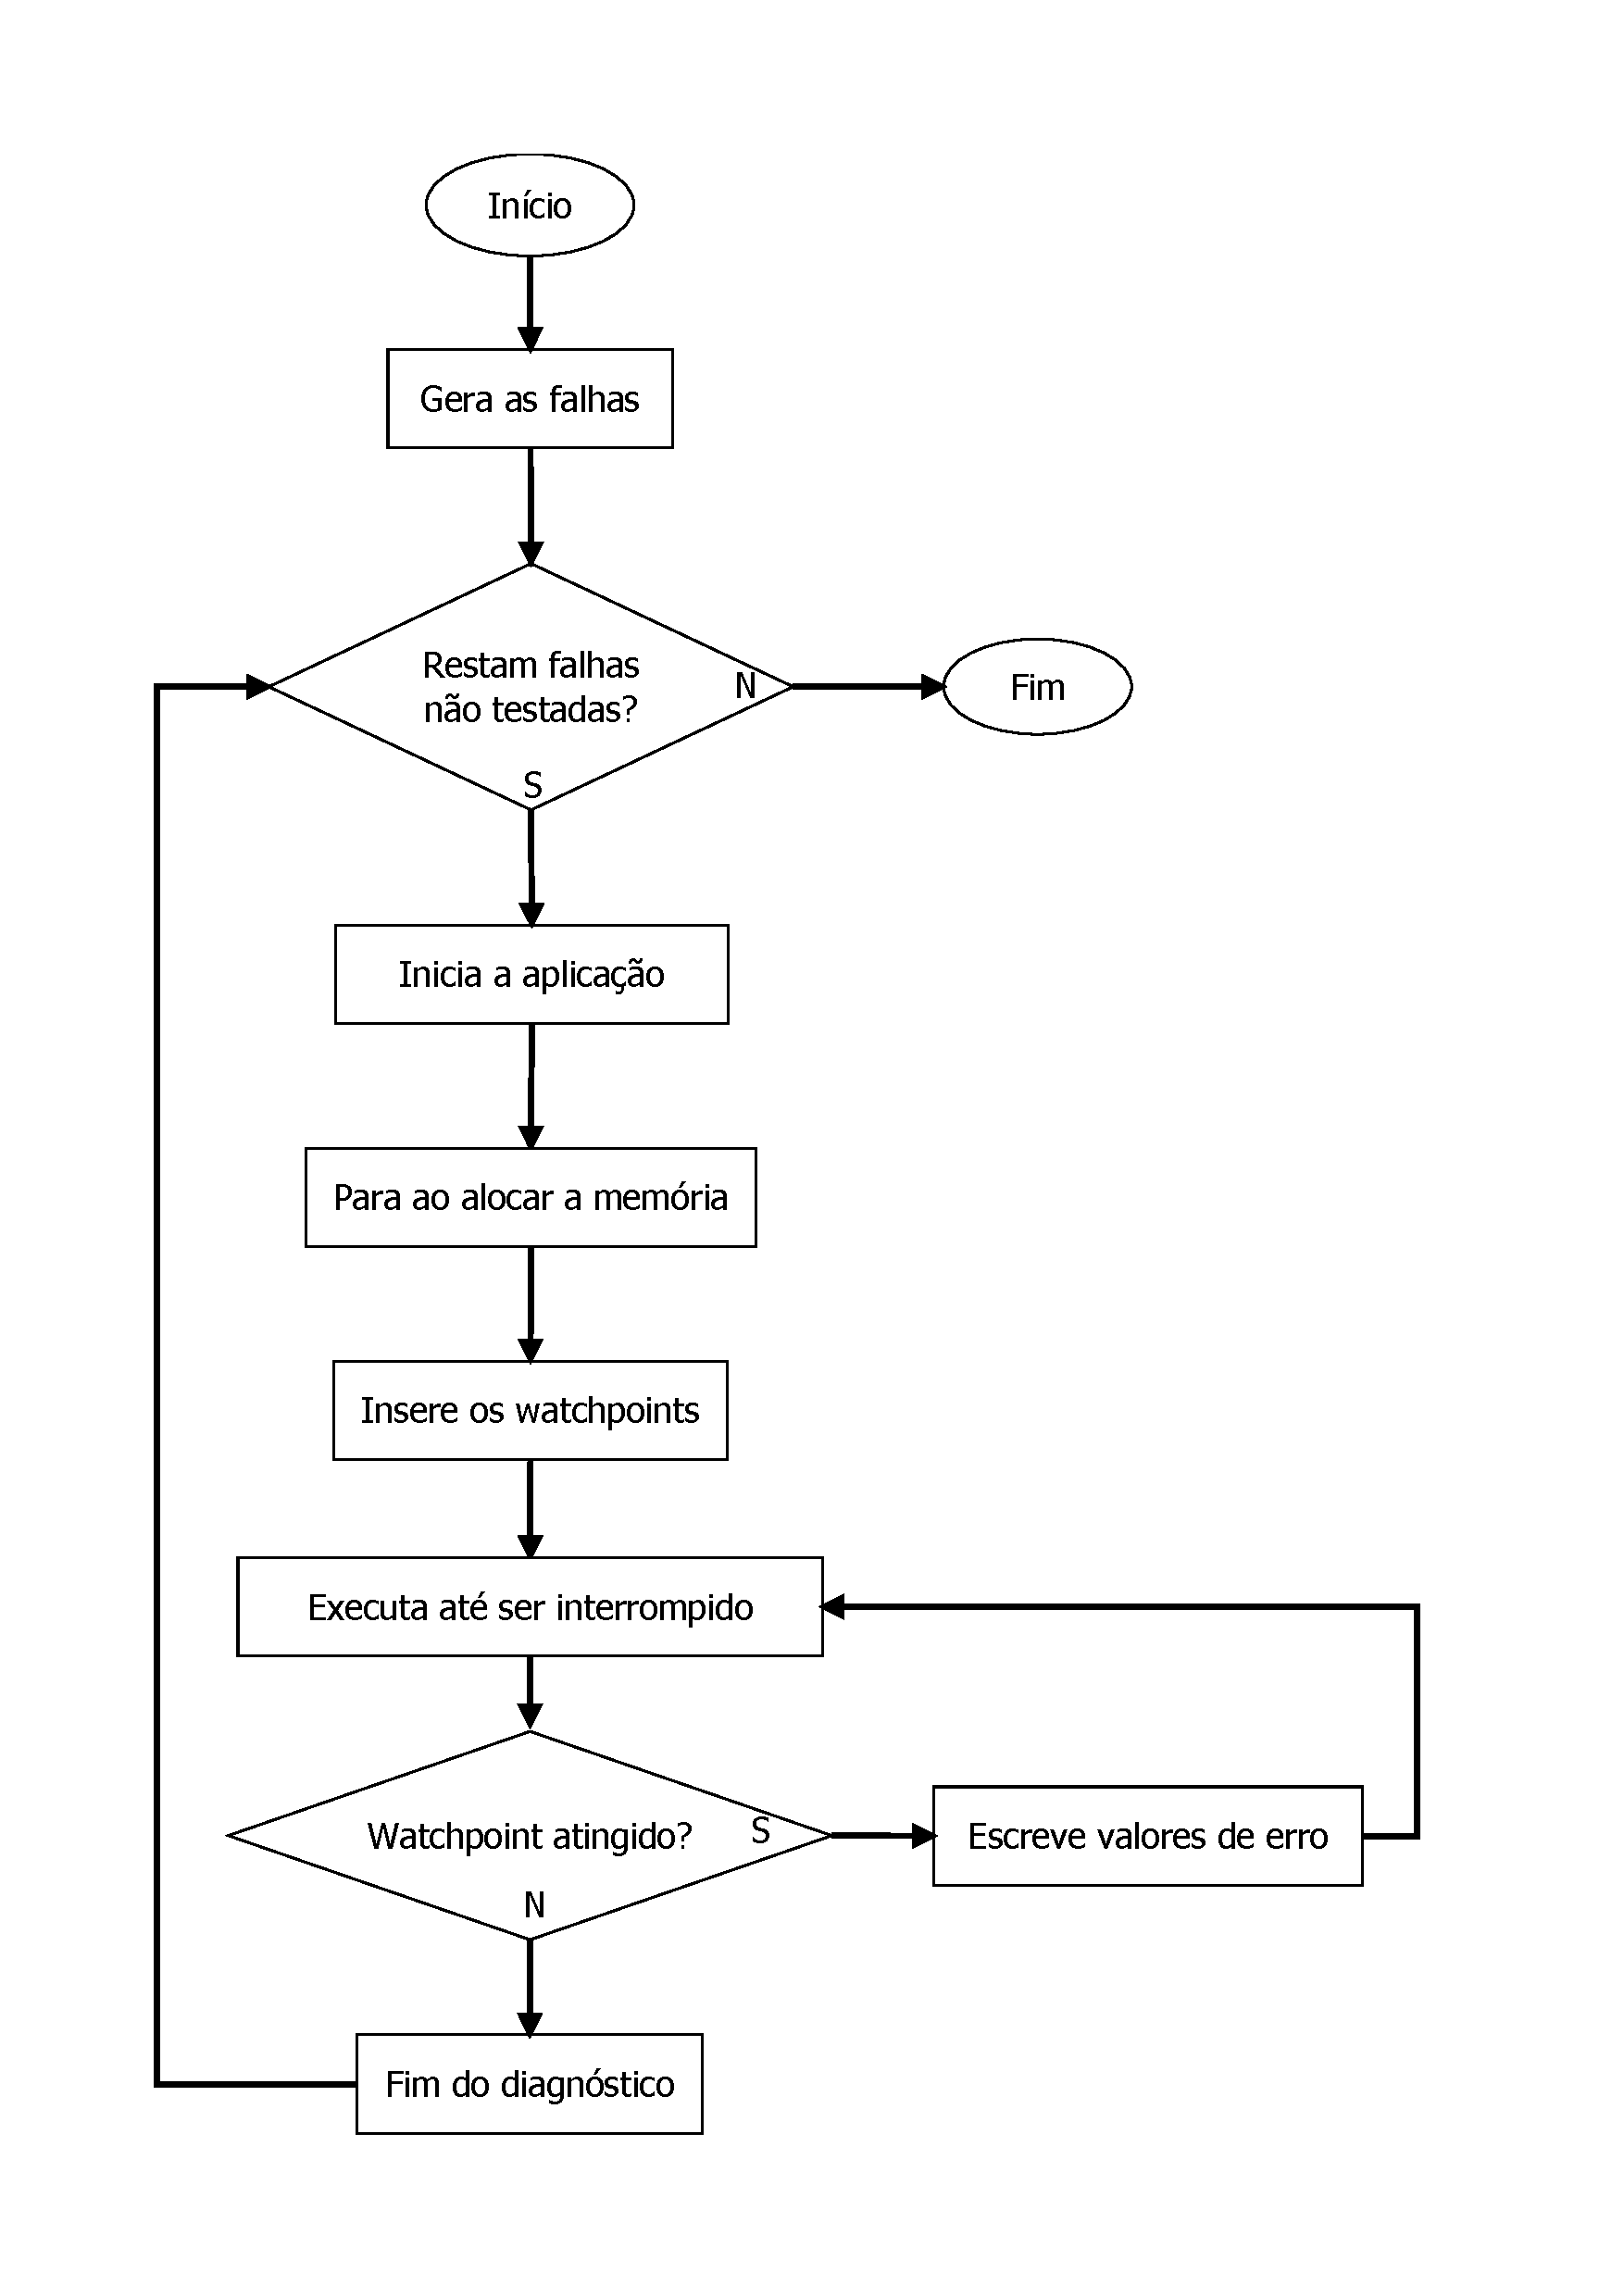
\includegraphics[width = 0.9 \linewidth]{figs/fluxo_sim.pdf}
\caption[Fluxograma do m�todo de inser��o de falhas]{Fluxograma do m�todo de inser��o de falhas.} \label{FIG:FLUXO_SIM}
\end{figure}

As falhas s�o geradas atrav�s de um \emph{script} que escreve arquivos com os modelos das falhas utilizando comandos pr�prios do \ac{GDB}. %Por exemplo, uma falha do tipo \ac{CF} entre o \emph{bit} 3 do endere�o 100 e o \emph{bit} 5 do endere�o 101 � representada por um \emph{script} com os seguintes comandos do \ac{GDB}:

%\begin{quote}
%set \$x = buffer[100] \& ($\sim$(1$\ll$3))
%
%set \$y = ((buffer[101] \& (1$\ll$5)) $\gg$ 5) $\ll$ 3
%
%set buffer[100] = \$x | \$y
%\end{quote}

Para otimizar o tempo de valida��o, as falhas s�o inseridas em conjuntos. A quantidade � limitada pelo m�ximo de \emph{watchpoints} que o processador utilizado suporta. Neste trabalho foi poss�vel inserir tr�s falhas a cada execu��o do ciclo maior da figura \ref{FIG:FLUXO_SIM}. O endere�o de cada uma � gerado a uma dist�ncia de 3 c�lulas da anterior, possibilitando que os arranjos da figura \ref{FIG:CELULAS_FALHAS} n�o se sobreponham. Assim, foram necess�rias 323 itera��es para cobrir todas as falhas testadas. A quantidade de mem�ria necess�ria para comportar $n$ falhas � de $4 \cdot n - 1$. Portanto, apenas 11 bytes s�o suficientes para comportar as falhas inseridas em uma itera��o. Por este motivo, a quantidade de mem�ria alocada pelo MDiag, durante este processo de valida��o, foi for�ada para o m�ximo de 1 MB, diminuindo bastante o tempo de teste de cada algoritmo.

O MDiag foi desenvolvido de modo a guardar em um arquivo de relat�rio todos os acontecimentos relevantes durante a sua execu��o, como a quantidade de mem�ria alocada, tempo de execu��o, falhas encontradas, etc. Estes relat�rios passaram por um tratamento autom�tico posterior para se obter os resultados relevantes. Estes resultados s�o apresentados e discutimos na pr�xima se��o. 
    %%% Se��o 3.4:
    \section{Teste em Ambientes Reais}
\label{SEC:REAL}

Al�m do ambiente de simula��o de falhas descrito na se��o anterior, o MDiag tamb�m foi submetido a situa��es de uso reais a fim de garantir sua utilidade pr�tica.

O acervo utilizado para teste foi composto por dez placas de mem�ria, algumas em perfeito funcionamento, outras com falhas. Metade delas possu�am encapsulamento \ac{SO-DIMM}, pr�prias para computadores de dimens�es reduzidas, como \emph{notebooks} e \emph{netbooks}, e as outras, encapsulamento \ac{DIMM}, geralmente usadas nos computadores pessoais comuns, estilo \emph{desktop}, ou em servidores.

Nesses testes, o MDiag confrontou dois \emph{softwares} de diagn�stico consagrados no mercado. O primeiro foi o \ac{LTT} \cite{LTT:2011}, desenvolvido pela PC-Doctor \cite{PCDOCTOR:2011} para os computadores da fabricante Lenovo. Na realidade este produto re�ne um conjunto de diagn�sticos que cobre quase todos os componentes da m�quina. O segundo foi o Memtest86+ \cite{MEMTEST:2011}, umas das ferramentas de diagn�stico de mem�ria mais abrangentes em termos de cobertura de falhas.

� importante ressaltar que o \ac{LTT} foi utilizado com o sistema operacional Windows, enquanto o Memtest86+ � uma ferramenta \emph{stand-alone} que executa diretamente de uma m�dia externa, como um CD ou \emph{pendrive} sem carregar nenhum \ac{SO}. Estas caracter�sticas influenciaram bastante nos resultados, pois afetam diretamente a quantidade de mem�ria testada.

O teste com cada ferramenta foi executado cinco vezes para cada m�dulo de mem�ria. Estas, por sua vez, foram etiquetadas cegamente, n�o havendo nenhum conhecimento pr�vio sobre a presen�a ou aus�ncia de falhas em cada uma delas.

Uma estimativa do tempo de execu��o de cada algoritmo implementado pelo MDiag foi elaborada com base na sua complexidade e levando em considera��o o \emph{overhead} das opera��es realizadas entre as escritas e leituras. Um algoritmo pode exigir apenas $10 N$ opera��es de acesso a mem�ria, mas para ser realizado ainda � necess�rio alocar mem�ria, executar checagens ap�s as leituras, incrementar o contador de endere�o, desalocar mem�ria, etc. Assim, o total de opera��es de uma implementa��o deve ser maior que o simples valor da complexidade.

A estimativa utilizou a f�rmula \ref{EQU:FUNCLOGIS}, na qual $C$ � a complexidade do algortimo e $O$ � um par�metro de tempo m�dio por opera��o, levando-se em conta alguns processamentos extras necess�rios. O valor de $O$ foi medido para cada algoritmo, individualmente, dividindo-se o tempo gasto para executar um elemento de teste pela quantidade de opera��es naquele elemento.

\begin{equation}
{T_{est} = C \cdot O}
\label{EQU:FUNCLOGIS}
\end{equation}


\section{Resumo do Cap�tulo}

Neste cap�tulo foram descritos os principais passos e medidas tomadas no desenvolvimento da aplica��o.
Tamb�m foi abordada a metodologia de valida��o elaborada para medir a efici�ncia dos algoritmos escolhidos.

No cap�tulo seguinte, s�o apresentados os resultados dos testes de inser��o de falhas utilizados para validar a ferramenta, al�m de medir o desempenho desta em rela��o a ferramentas do mercado.

